%% figure 객체: fig:measure-predict — 교전 구성·결과 측정·예측·평가의 흐름과 두 모형(승률 평가기, 방향 예측기)의 구분.
%% 원본 figures/measure_predict.png. 그림 안의 설명 문장(제목, 부제, 교전 구성 문장, 교전 후 상태 문장, fold 평가기 각주)은
%% 5.1절 본문으로 옮기고 이미지에서 지웠다.
%% 원본에서 남은 수정: "Same observed SVI labels" -> "Same SVI labels"; "Baseline PT", "Brier(PT)" -> PT_flex;
%% "evaluator V" -> V-hat; 막대 색 범례 또는 단색; 글자 약 1.5배(가로 전면에서 주요 라벨 약 6-7 pt, 작은 주석 약 4-5 pt).
\begin{sidewaysfigure}
  \centering
  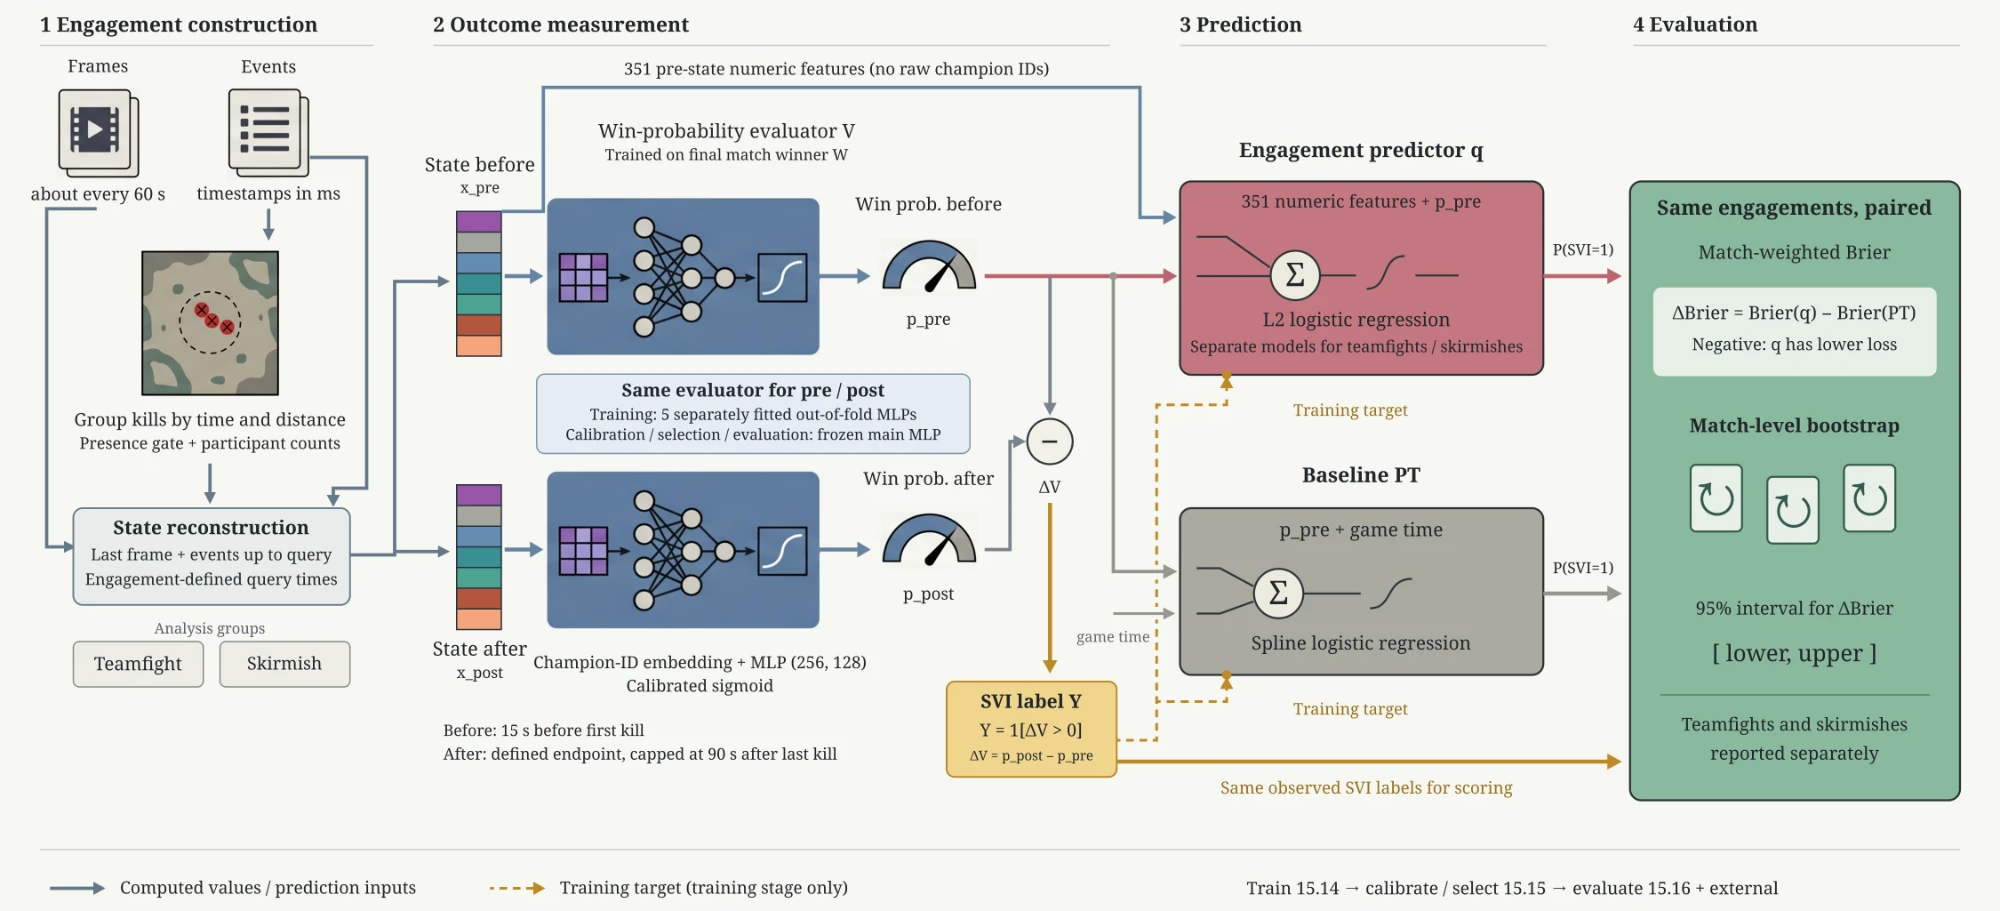
\includegraphics[width=\linewidth]{figures/measure_predict.png}
  \caption{교전 결과의 측정과 방향 예측}
  \label{fig:measure-predict}
\end{sidewaysfigure}
